% Generated from saved forward-only traces by make_reference_trace.py.
\subsection{Forward-reference diagnostic without NMS or masks}
\label{app:seg-forward-reference}
A subsequent prospective diagnostic records the forward-reference workload alone on the same CPU, model and one fixed clean image. Two fresh processes each execute 12 blocks of three fixed warmup forwards and 15 timed forwards: one continuous cadence and one with a two-second pause between blocks. The registered order is continuous first. PDH is recorded after every timed forward, and each output is released after both clocks. All 360 samples complete, pin-load checks pass, and all 45 application affinities are restored before analysis.
The continuous trace flags 4/12 block medians and the paused trace flags 2/12 against their own first-block median using the descriptive 3\% threshold; every flagged block is faster. Thus reference drift exceeding this threshold is observed even without NMS or mask work. This does not uniquely identify the mechanism of the earlier component failures. There is one process per cadence and the fixed order confounds cadence with session/time; the flag counts are not evidence that pausing improves stability. No CI, p-value, A/A MDE or attack qualification is inferred, no baseline is replaced, and the finite protocol stops without retry.
\begin{figure*}[t]\centering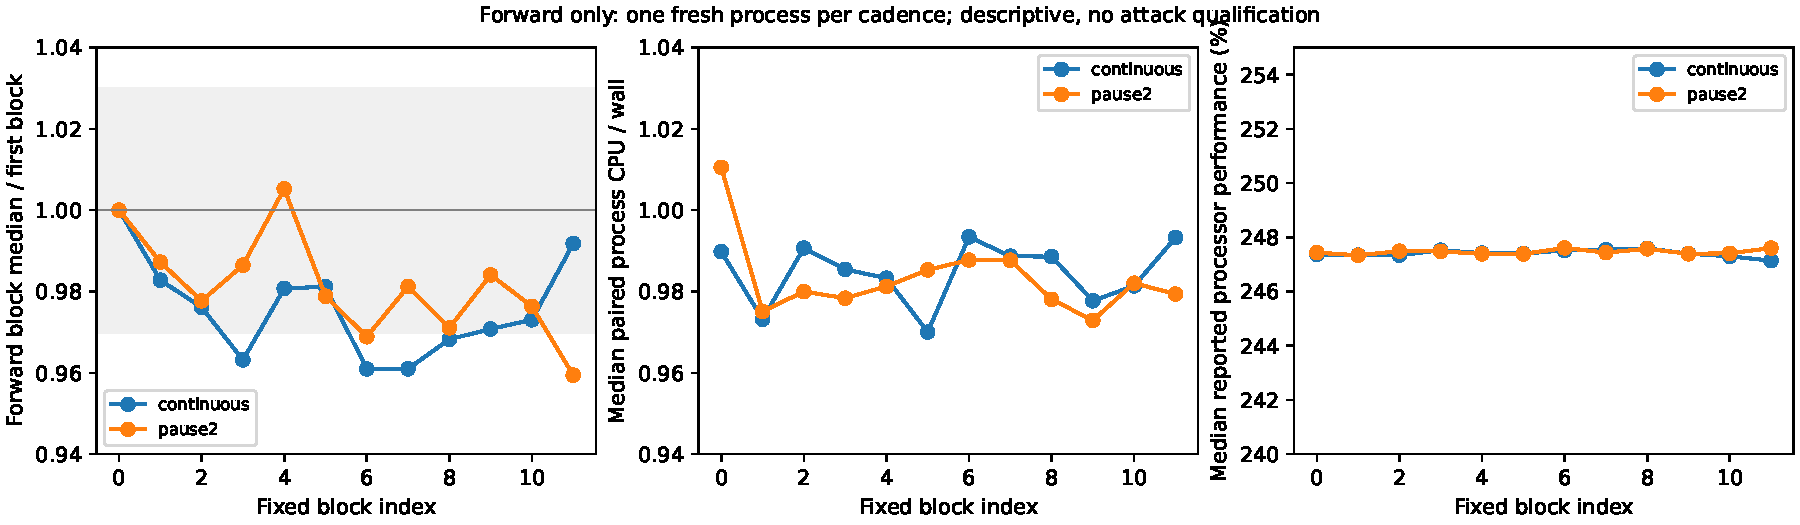
\includegraphics[width=.98\textwidth]{segmentation_extension/laptop_reference_trace.pdf}\caption{Forward-only diagnostic: block wall-median ratios, median paired process-CPU/wall values, and median reported processor-performance counter. Shading marks the descriptive 3\% band. Interval counters and quantized process CPU do not identify thermal, clock, cache or scheduling causes.}\label{fig:seg-forward-reference}\end{figure*}
The initial runtime, pin-load and cache context differs from the component workload. These controls retain all observations, supply no ARM or service-denial result, and do not promote either previously failed component contrast.
